
\documentclass[conference]{IEEEtran}

\usepackage[style=numeric, uniquename=full, sorting=none,backend=biber, natbib=true]{biblatex}

%se importan las configuraciones custmizdas realizadas.
\addbibresource{../book/referencias.bib}

\usepackage[spanish]{babel}
\usepackage[utf8]{inputenc}

% *** GRAPHICS RELATED PACKAGES ***
%
\usepackage[pdftex]{graphicx}


% *** MATH PACKAGES ***
%
\usepackage{amsmath,amsthm}
\usepackage{textcomp}

% *** SPECIALIZED LIST PACKAGES ***
%
%\usepackage{algorithmic}



% *** ALIGNMENT PACKAGES ***
%
%\usepackage{array}
%\usepackage{mdwmath}
%\usepackage{mdwtab}

%\usepackage{eqparbox}
\usepackage{threeparttable}
\usepackage{caption}
\usepackage{subcaption}
%\usepackage[caption=false]{caption}
%\usepackage[font=footnotesize]{subfig}

%\usepackage[caption=false,font=footnotesize]{subfig}

% *** FLOAT PACKAGES ***
%
%\usepackage{fixltx2e}
%\usepackage{stfloats}

\newcommand{\figref}[1]{Figura \ref{#1}}
\newcommand{\tabref}[1]{Tabla \ref{#1}}
\newcommand{\secref}[1]{sección \ref{#1}}
\newcommand{\algref}[1]{Algoritmo \ref{#1}}

% correct bad hyphenation here
\hyphenation{}


\begin{document}
%
% paper title
% can use linebreaks \\ within to get better formatting as desired
\title{Modelo predictivo de focos de dengue aplicado a Sistemas de Información Geográfica}


% author names and affiliations
% use a multiple column layout for up to three different
% affiliations
\author{\IEEEauthorblockN{Maximiliano Báez González}
    \IEEEauthorblockA{Facultad Politecnica \\
    Universidad Nacional de Asunción\\
    Email: maxibaezpy@gmail.com}
}
% make the title area
\maketitle

\begin{abstract}
%\boldmath
El Dengue es una enfermedad viral transmitida por el mosquito del Aedes aegypti. En Paraguay las autoridades sanitarias llevan a cabo acciones para la vigilancia entomológica con el fin monitorear la densidad vectorial en zonas endémicas y no endémicas, mediante técnicas basadas en utilización de indices tradicionales. Actualmente existen numerosos métodos e indicadores más prácticos, eficientes y económicos para determinar las poblaciones de Aedes aegypti como larvitrampas y ovitrampas. La información regionalizada obtenida de los métodos de muestreo, como larvitrampas y ovitrampas, puede ser combinada con información ambiental, demográfica o epidemiológica, con el fin de obtener modelos detallados que tengan la capacidad de monitorear, simular el comportamiento del vector y en consecuencia, predecir una posible epidemia del dengue. En este trabajo presenta el diseño e implementación de un modelo predictivo para identificar focos de infestación del vector del dengue. El modelo es implementado como un simulador del proceso evolutivo de la ecología del vector, compuesto de un conjunto de submodelos que buscan estimar la tasa de desarrollo, mortalidad, reproducción y dispersión del vector del dengue ante las variaciones climáticas a las que es sometido, donde la población inicial es generada a partir de la información obtenida de las larvitrampas, con el fin de generar información suficiente para contribuir con la detección temprana de posibles brotes epidemiológicos.
\end{abstract}

\begin{IEEEkeywords}
Aedes, dengue, vectores de enfermedades, modelos estadísticos, mapa de riesgo,vigilancia  epidemiológica, SIG, Dinámica de la población de Aedes aegypti.
\end{IEEEkeywords}

% For peerreview papers, this IEEEtran command inserts a page break and
% creates the second title. It will be ignored for other modes.
\IEEEpeerreviewmaketitle

%introduccion
%----------------------------1----------------------------------
\begin{frame}[t]{Motivación y Definición del Problema.}
  \begin{center}
    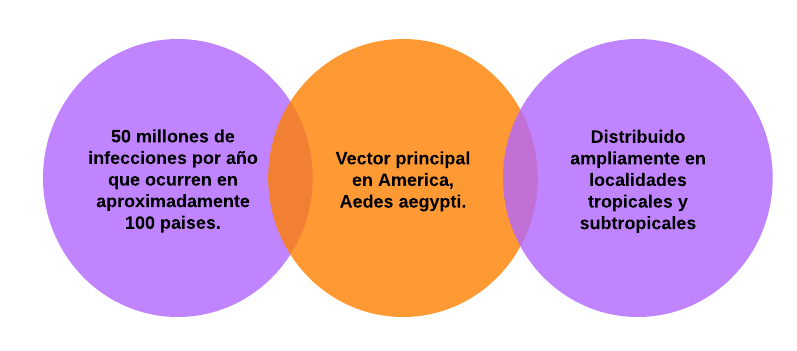
\includegraphics[width=10cm]{./graphics/dengue-intro.png}
  \end{center}
\end{frame}

%----------------------------2----------------------------------

\begin{frame}[t]{Motivación y Definición del Problema.\\\textit{Criaderos del Aedes aegypti.}}
\begin{center}
    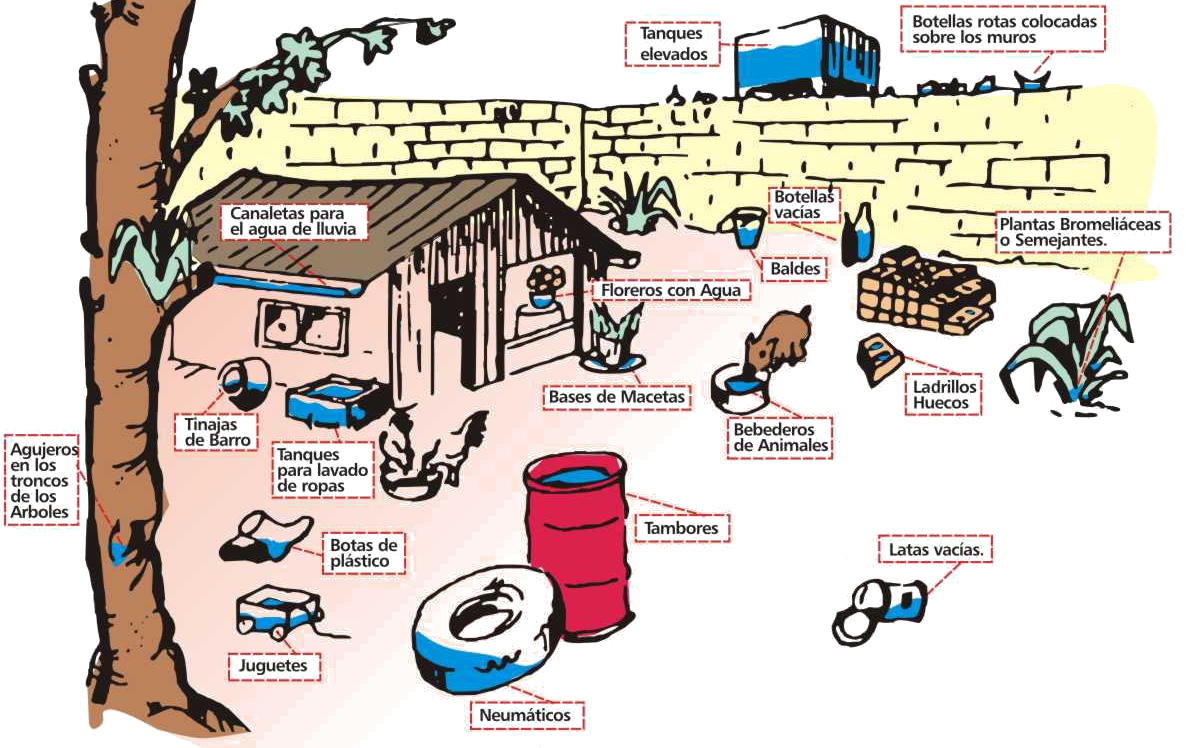
\includegraphics[width=9cm]{./graphics/criaderos.jpg}
    \end{center}
\end{frame}

%----------------------------3----------------------------------


%----------------------------4----------------------------------

\begin{frame}[t]{Motivación y Definición del Problema.\\\textit{Dengue en Paraguay.}}
  \begin{center}
    \begin{itemize}
    \item El Paraguay desde el año 2009 es considerado un país endémico.

    \item El clima, subtropical, favorece la aparición y desarrollo del dengue.

    \item Se realizan actividades de monitoreo del comportamiento el vector mediante técnicas tradicionales de vigilancia.

    \item Se utilizan técnicas de control vectorial, como fumigación, para la disminución de las poblaciones de mosquitos.

    \item En las últimas décadas se han observado un crecimiento considerable de las notificaciones de posibles casos de dengue, algunas con derivaciones fatales.
    \end{itemize}
  \end{center}
\end{frame}

%----------------------------5----------------------------------

\begin{frame}[t]{Motivación y Definición del Problema.\\\textit{Dengue en Paraguay.}}
  \begin{center}
  \begin{table}
      \begin{minipage}{\textwidth}
          \begin{center}
          \caption{Histórico de casos de dengue notificados, confirmados y con derivación fatal en Paraguay.}
          \begin{tabular}{l c c r r}
              \hline
              Año & Periodo (inicio / fin) & Notificados & Confirmados & Muertes\\
              \hline
              \hline
              2014 & 29-12-13 / 31-05-14 & 10.541 & 1.052 & 2\\
              2013 & 30-12-12 / 21-12-13 & 153.793 & 131.306 & 70\\
              2012 & 01-01-12 / 22-12-12 & 37.815 & 30.588 & 11\\
              2011 & 03-01-11 / 29-12-11 & 53.397 & 42.264 & 62\\
              2010 & 11-10-09 / 25-12-10 & 21.951 & 13.760 & --$^a$
          \end{tabular}
          \footnotetext[1]{No se encontraron datos sobre muertes en el periodo.}
          \end{center}
      \end{minipage}
  \end{table}
  \end{center}
\end{frame}

%----------------------------6----------------------------------

\begin{frame}[c]{Motivación y Definición del Problema.\\\textit{Vigilancia Entomológica en Paraguay.}}

    \begin{itemize}
      \item La Vigilancia Entomológica es un proceso orientado al levantamiento de información sobre la distribución del vector.

      \item Para estimar la densidad del vector, la OMS ha recomendado los siguientes indicadores entomológicos : Índice de Casa, Índice de Recipiente e Índice de Breteau.

      \item Sólo son recomendados para detectar la calidad de las acciones realizadas por el personal de control larvario.

      \item Las autoriadades sanitarias del Paraguay utilizan estos índices para estimar la densidad poblacionál del vector.

    \end{itemize}
\end{frame}

\begin{frame}[c]{Motivación y Definición del Problema.\\\textit{Vigilancia Entomológica en Paraguay.}}
\begin{itemize}
      \item Actualmente son considerados, por la OMS, como una pobre indicación de la producción de mosquitos adultos.

      \item No reflejan la asociación que existe entre las densidades de mosquitos y los tipos de recipientes.

      \item Proporcionan poca o nula información de aquellas viviendas en las que existe un mayor riesgo de presencia de mosquitos.

      \item Existen numerosos métodos e indicadores más prácticos, eficientes y económicos, como larvitrampas y ovitrampas\footnote{Centro Nacional de Programas Preventivos y Control de Enfermedades. \textit{Guía para la Vigilancia Entomológica con Ovitrampas}. Oct 2013.\\}.

    \end{itemize}
\end{frame}

%----------------------------7----------------------------------

\begin{frame}[t]{Motivación y Definición del Problema.\\\textit{Larvitrampas.}}
  \begin{center}
    \begin{columns}[c]
        \begin{column}[c]{3cm}
          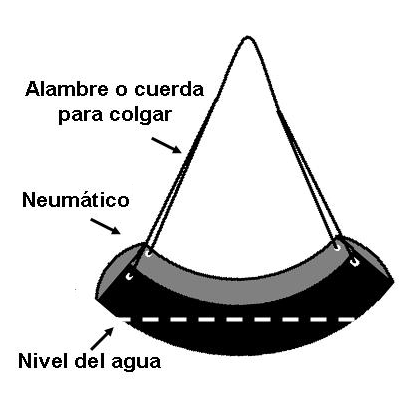
\includegraphics[width=\textwidth]{../book/anexos/graphics/disenho-1.png}

          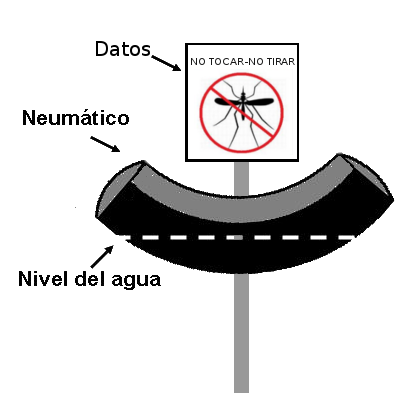
\includegraphics[width=\textwidth]{../book/anexos/graphics/disenho-2.png}
        \end{column}
        \begin{column}[c]{7cm}
          \begin{itemize}
            \item Criadero artificial y controlado.
            \item Se basan en la detección del vector en su etapa larval.
            \item Brinda información sobre los patrones de actividad espacial y estacional de ovipostura.
            \item Permiten reconocer las condiciones climáticas favorables para la eclosión y desarrollo larvario.
            \item Materiales reciclados como materia prima.
          \end{itemize}
        \end{column}
      \end{columns}
  \end{center}
\end{frame}

\begin{frame}[t]{Motivación y Definición del Problema.\\\textit{Larvitrampas.}}
  \begin{center}
    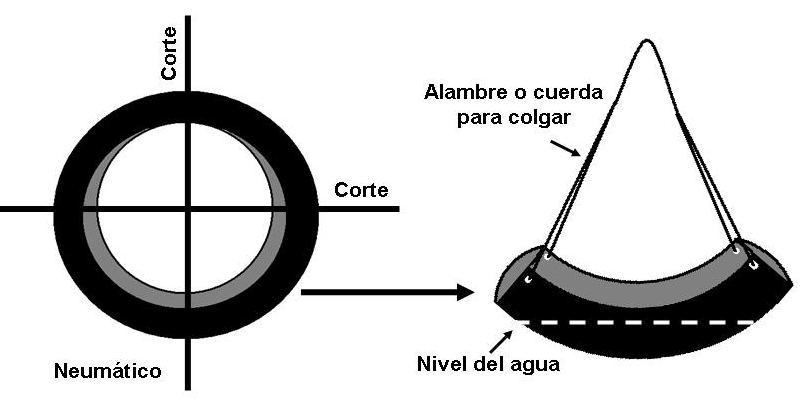
\includegraphics[width=9cm]{../book/anexos/graphics/construccion-larvitrampa.png}
  \end{center}
\end{frame}

%----------------------------6----------------------------------
\begin{frame}[t]{Motivación y Definición del Problema.\\\textit{La problemática del dengue en Paraguay.}}
  \begin{itemize}

    \item Las autoridades sanitarias del Paraguay no cuentan con datos computables, geográficamente, referentes al dengue, que permitan realizar análisis estadísticos y espaciales.

    \item Se deben diseñar y desarrollar herramientas para la recolección de la información, para su posterior análisis.

    \item Se deben optar por nuevas metodologías que permitan generar información para el análisis sin la necesidad de grandes requerimientos.

    \item Las larvitrampas y ovitrampas permiten generar información regionalizada sobre el estado y la distribución de la población del vector.

  \end{itemize}
\end{frame}


%Materiales y metodos
\section{Modelo propuesto}
Los métodos de muestreo, como larvitrampas y ovitrampas resultan eficientes y económicos para
determinar determinar la distribución espacial y temporal de Aedes aegypti y otros mosquitos
\cite{dengueUruguayCap1, cenaprece2013}. La distribución geográfica de larvitrampas, consideradas
como puntos de control, permiten generar información regionalizada sobre el estado de las
poblaciones del vector \cite{NINO2011}, en donde esta información puede ser combinada con
información ambiental, demográfica o epidemiológica, con el fin de obtener modelos detallados que
tengan la capacidad de monitorear, simular el comportamiento del vector y en consecuencia,
predecir una posible epidemia del dengue.

El modelo considera un espacio bi-dimensional, con un sistema de coordenadas geográficas $(x,y)$,
para expresar todas las posiciones sobre el plano, correspondientes a la longitud y latitud. Si
consideramos a $m_{i}$ como a un individuo que se encuentra en una etapa del ciclo de vida del
Aedes aegypti, correspondiente a una población de mosquitos, entonces, $m_{i}(x,y)$ representa a
$m_{i}$ en las coordenadas geográficas $(x,y)$.

La evolución de las poblaciones, se ven afectadas por los siguientes eventos: muerte de huevos,
eclosión de huevos, muerte de larvas, emergencia de pupas, muerte de pupas, emergencia de adultos,
muerte de adultos, ovipostura de hembras nulíparas\footnote{Hembras que no han ovipuesto.},
ovipostura de hembras paridas\footnote{Hembras que han ovipuesto al menos una vez.} y dispersión
de los adultos (machos y hembras). Según \cite{otero2006stochastic} los eventos se producen a
tasas que dependen no sólo de valores de la población, sino también de la temperatura, que a su
vez es una función de tiempo, por lo tanto, la dependencia de la temperatura introduce una
dependencia del tiempo en las tasas de eventos.

\subsection{Tasas de desarrollo}
En el modelo se cuenta con 4 tasas de desarrollos correspondientes a : la eclosión de huevos,
emergencia a pupas, emergencia a adultos y el ciclo gonotrófico. Estos valores son obtenidos
mediante el modelo no lineal de Sharpe y DeMichele, presentado en \cite{sharpe1977reaction}, para
procesos poiquilotermos\footnote{La poiquilotermia o ectotermia es un término aplicado a ciertos
animales con temperatura corporal variable}, donde el proceso de maduración es controlado por
una enzima que actúa en un rango de temperatura determinado, la enzima se desactiva a las bajas
temperaturas, y altas. Schoolfield presentó, en \cite{schoolfield1981non}, un versión simplificada
del modelo de Sharpe y DeMichele con inhibición de altas temperaturas, con una única alta
temperatura de desactivación.

\begin{equation} \label{eq:schoolfield}
   R(k)  = R(298K) *\cfrac{ \cfrac{k}{298K} *
    exp \Bigg[
            \cfrac{\Delta H_{A}}{R} \bigg(\cfrac{1}{298K} - \cfrac{1}{k}\bigg)
        \Bigg]}
    {1 + exp\Bigg[\cfrac{\Delta H_{H}}{R} \bigg(\cfrac{1}{T_{1/2}}- \cfrac{1}{k}\bigg)\Bigg] }
\end{equation}

Donde $R(k)$ representa la tasa de desarrollo media ($dias^{-1}$) para una temperatura $K$,en la
escala de Kelvin; $T_{1/2}$ es la temperatura cuando la mitad de la enzima se desactiva, debido a
la alta temperatura, mientras que $H_{A}$, $H_{H}$ y $H_{L}$ son entalpías termodinámicas
características del organismo, y $R$, igual $1,987202$ $cal/K.mol$, es la constante universal de
los gases. Los parámetros $R(298K)$, $H_{A}$, $T_{1/2}$, y $H_{H}$ son estimados mediante la
de regresión no lineal de Wagner, presentado en \cite{wagner1984modeling}. Según
\cite{otero2006stochastic}, el modelo simplificado de Schoolfield, es lo suficientemente
flexible para el ajuste de los datos biológicos disponibles. Los parámetros deben calcularse para
cada etapa de desarrollo, una vez determinados, la ecuación puede utilizarse para calcular tasas
de desarrollo a cualquier temperatura \cite{rueda1990temperature}.

\subsection{Zonificación}
\label{subsec:cap4-zonificacion}
Cada entorno puede contar con factores que lo hagan más o menos apto para el desarrollo,
mortalidad, alimentación, dispersión, y reproducción de individuos. Con el fin de
simplificar ciertos aspectos muy específicos que se encuentran fuera del alcance de este trabajo,
se realizan ciertas hipótesis generales, justificadas para este caso de aplicación, pero puede
requerir una revisión en caso general. Estas hipótesis son, los valores observados en un
conjunto de puntos de control, pertenecientes a una zona, permiten la caracterización de dicha
zona como más o menos apta para desarrollo, mortalidad, alimentación, dispersión, y reproducción de
individuos. También consideramos que el tamaño de la zona, y por ende la cantidad de puntos de
control que pertenecen a ella, influye en la caracterización de las zonas.

Para determinar el tipo de zona de un individuo $m_{i}$ ubicado en $(x,y)$, primero se estima la
densidad relativa de larvas, para $m_{i}(x,y)$, utilizando interpolación espacial y posteriormente
se la clasifica utilizando una escala. Si consideramos a $u(x,y)$ el valor interpolado para
$m_{i}(x,y)$, entonces la densidad relativa de larvas de $m_{i}(x,y)$ es igual a $u(x,y)$.

La forma general de encontrar un valor interpolado $u$ en un punto $(x,y)$ basado en un conjunto de
muestras $u_i = u (x_i)$ para $i = 0,1, ..., N$ utilizando IDW, es una función de interpolación:

\begin{equation}\label{eq:interpolacion-idw}
 u(x,y) = \sum_{i=1}^{N} w_i(X) * u_{i}
\end{equation}

Donde :
\begin{equation}
w_i(X) =  \dfrac{d(X, X_i)^{-p}}{\sum_{j=1}^{N} d(X, X_i)^{-p}}
\end{equation}

Siendo $d(X, X_i)$ una función que determina la distancia existente entre $X$ y $X_{i}$, donde $p$
es el exponente de ponderación.  El valor estimado de $u(x,y)$ es utilizado para clasificar la
zona como \textit{Pésima}, \textit{Mala}, \textit{Regular}, \textit{Buena} u \textit{Óptima} con
influencia positiva el desarrollo, alimentación, dispersión, y reproducción de individuos y
negativamente para la mortalidad.

\begin{table}[!hptb]
\begin{threeparttable}
    \begin{minipage}[b]{0.5\textwidth}
    \caption{\label{tab:cap4-puntaje-zona} Escala de clasificación de las zonas de acuerdo a la densidad relativa de larvas.}
    \footnotesize
    \begin{tabular}{l c c c c}
        \hline \\
                     & Mínimo\tnote{a} & Máximo\tnote{a} & Hembras     & Hembras \\
        Tipo de zona & $u(x,y)$   & $u(x,y)$   & Adultas\tnote{b} & Reproductivas \tnote{c}\\
        \hline
        \hline\\
        Pésima  & 0  & 19 & 8  & 5 \\
        Mala    & 20 & 35 & 15 & 10\\
        Regular & 36 & 51 & 22 & 15\\
        Buena   & 52 & 69 & 30 & 20\\
        Óptima  & 70 & --\tnote{d} & --\tnote{d} & --\tnote{d}\\
        \hline
    \end{tabular}
    \begin{tablenotes}[flushleft]\footnotesize
    \item[a]{Rango mínimo y máximo de $u(x,y)$ permitido para el tipo de zona.}
    \item[b]{Cantidad máxima de hembras adultas, al final del periodo de desarrollo.}
    \item[c]{Cantidad de hembras adultas con capacidad de oviponer.}
    \item[d]{No se estableció un límite superior para las zonas óptimas. }
    \end{tablenotes}
    \end{minipage}
    \end{threeparttable}
\end{table}

En la \tabref{tab:cap4-puntaje-zona} se pueden observar los rangos definidos para cada tipo de
zona, en donde $u$ es la densidad relativa de larvas en las coordenadas $(x,y)$. Los límites para
las zonas fueron determinados clasificando los valores, de las hembras reproductivas en, grupos
múltiplos de cinco. No se estableció un límite superior para las zonas óptimas debido a que los
valores mayores a el mínimo establecido, 70 larvas por dispositivo, pertenecen a la misma categoría

\subsection{Mortalidad}
\label{subsec:cap4-mortalidad}
La mortalidad de los individuos depende de la etapa del ciclo de desarrollo en el que se encuentren
los individuos de una población.

\subsubsection{Mortalidad de huevos}
La tasa de mortalidad de los huevos se encuentra definida como una constante, $me = 0.01$,
$1/\text{días}$, independiente de la temperatura \cite{otero2006stochastic}.

\begin{equation}
    M_{H(x,y)} = me * H(x,y)
\end{equation}

Donde $M_{H(x,y)}$ es la cantidad de huevos que deben ser eliminados de la población $H(x,y)$.

\subsubsection{Mortalidad de larvas}
La mortalidad de las larvas, según \cite{otero2006stochastic}, se encuentra dividida en dos
contribuciones. La primera contribución representa la mortalidad natural bajo óptimas condiciones
y se encuentra influenciada únicamente de la temperatura \cite{otero2006stochastic}. Esta tasa se
encuentra definida por :

\begin{equation}
\label{eq:mortalidad-natural-larvas}
    ml(k) = 0.01 + 0.9725 * exp\bigg( \frac{-(k - 278)}{2.7035}\bigg)
\end{equation}

La segunda contribución es la mortalidad denso dependiente de las larvas \cite{otero2006stochastic}
. Este mecanismo de regulación puede estar relacionado con procesos concurrentes, como las
limitaciones de los alimentos, las interacciones químicas, presencia de depredadores
especializados en el sitio de reproducción y mucho más \cite{otero2006stochastic}. Esta se
encuentra definida por :

\begin{equation}
  \alpha (x,y) = \alpha _{0}/BS(x,y)
\end{equation}

Donde $\alpha _{0}$ está asociado a la capacidad de carga de un solo lugar de reproducción y
$BS(x,y)$ es el número de sitios de reproducción en $(x,y)$. El valor de $\alpha _{0}$ puede
ajustado a los valores observados en la región que se está simulando. Se considera que el valor de
$BS(x,y)$ se encuentra influenciado por $u(x,y)$, de ese modo a medida que $u(x,y)$ varíe, lo debe
hacer el valor de $BS(x,y)$. Para el cálculo de $BS$ relativo a $(x,y)$ se utiliza el método
interpolador de Lagrange.

\begin{equation}
\label{eq:sitios-reproduccion-x-y}
    bs(u(x,y)) = \sum_{i=0}^{n} bs_{i} * l_{i}(u(x,y))
\end{equation}

donde $l_j(u(x,y))$ son los llamados polinomios de Lagrange, que se calculan de este modo:

\begin{equation}
\label{eq:sitios-reproduccion-x-y}
    l_{i}(u(x,y)) = \prod_{j \neq i} \cfrac{u(x,y) - u_{j}}{u_{i} - u_{j}}
\end{equation}

Consideramos un polinomio de tercer grado, con los parámetros $u_0$, $u_1$ y $u_2$ igual a $19$,
$51$ y $70$, correspondientes a zonas del tipo \textit{Pésima}, \textit{Regular} y \textit{Óptima}.
Los valores, $bs_{min}$, $bs_{med}$ y $bs_{max}$ respectivamente, estos son parámetros
configurables del modelo donde $bs_{min}$ representa el menor $BS$ observado, $bs_{max}$
representa el mayor $BS$ observado y $bs_{med}$ es el valor medio existente entre $bs_{max}$ y
$bs_{min}$.

Tomando ambas contribuciones, la mortalidad natural bajo óptimas condiciones y la denso
dependiente, la mortalidad de las larvas queda definida como :
\begin{equation}
    M_{L(x,y)}(k) = ml(k) * L(x,y) + \alpha (x,y) * L(x,y) * (L(x,y) - 1)
\end{equation}

Donde $M_{L(x,y)}$ es la cantidad de larvas que deben ser eliminadas de la población $L(x,y)$.

\subsubsection{Mortalidad de las pupas}
La tasa de mortalidad de las pupas se encuentra definida como una función influenciada únicamente
de la temperatura \cite{otero2006stochastic}.

\begin{equation}
\label{eq:mortalidad-natural-pupas}
    mp(k) = 0.01 + 0.9725 * exp\bigg( \frac{-(k - 278)}{2.7035}\bigg)
\end{equation}

Además de la mortalidad diaria en la fase de pupa, existe una importante mortalidad adicional
asociada con la emergencia sin éxito de adultos, solo el 83 \%  de las pupas alcanzan la maduración
y emergerán como mosquitos adultos, por lo tanto, el factor de supervivencia es de $ef = 0.83$
\cite{otero2006stochastic}.

\begin{equation}
    M_{P(x,y)}(k) = P(x,y) * (mp + (1 - ef) * R(k))
\end{equation}

Donde $M_{P(x,y)}$ es la cantidad de pupas que deben ser eliminadas de la población $P(x,y)$.

\subsubsection{Mortalidad de adultos}
La tasa de mortalidad de los adultos se encuentra definida como una constante, $ma = 0.09$,
$1/\text{días}$, independiente de la temperatura \cite{otero2006stochastic}.

\begin{equation}
    M_{A(x,y)} = ma * A(x,y)
\end{equation}

Donde $M_{A(x,y)}$ es la cantidad de adultos que deben ser eliminados de la población $A(x,y)$.

\subsection{Madurez y cambio de estado}
La madurez de los individuos pertenecientes a las poblaciones de $H(x,y)$, $L(x,y)$ y $P(x,y)$
indica la proximidad de que estos alcancen el siguiente estado de su etapa de desarrollo. Sea
$R(k_{i})$ la tasa de desarrollo de un individuo para una temperatura de $k_{i}$ Kelvin en un
instante $i$, se considera que ha alcanzado su máximo nivel de madurez y se encuentra listo para
pasar al siguiente estado de su cuando $\sum_{i=0}^{N} R(k_{i}) \geq 1$ , en donde $N$ es la
cantidad de días que le toma al individuo pasar de un estado a otro. Para $R(k)$ se se aplican los
parámetros correspondientes al estado actual del individuo.

\subsection{Ciclo gonotrófico y Ovipostura}
El ciclo gonotrófico de los mosquitos es el nombre que se le adjudicó al período que existe desde
que el mosquito realiza una alimentación sanguínea - ovipostura - hasta una nueva alimentación.
Como se mencionó anteriormente, la tasa de desarrollo del ciclo gonotrófico puede estimarse
mediante la versión simplificada del modelo de Sharpe y DeMichele \cite{sharpe1977reaction},
propuesta por Schoolfield en \cite{schoolfield1981non}.

Sea $R(k_{i})$ la tasa de desarrollo del ciclo gonotrófico de una hembra (nulípara o parida), para
una temperatura de $k_{i}$ Kelvin en un instante $i$, se considera que un día es de ovipostura si
se cumple $\sum_{i=0}^{N} R(k_{i}) \geq 1$, en donde $N$ es la duración en días del ciclo
gonotrófico de la hembra adulta. Para $R(k)$ se aplican los parámetros correspondientes a hembras
nulíparas y paridas de acuerdo al estado de la hembra. En \cite{edman1987host} se observó que
hembras nulíparas de Aedes aegypti poseen un proceso de digestión más lento en las hembras paridas
y por ende el ciclo gonotrófico de las mismas tiende a ser más largo. La cantidad de huevos en
cada oviposición, luego de las alimentaciones sanguíneas correspondientes, varía entre 30 y 100
unidades \cite{luevano1993ciclo, beltran2001bionomia,cabezas2005dengue}.

\subsection{Vuelo y dispersión}
El Aedes aegypti es un mosquito doméstico que generalmente esta confinado a las casas donde se
cría \cite{luevano1993ciclo}, tiende a permanecer físicamente en donde emergió, siempre y cuando
no exista algún factor que la perturbe o no disponga de huéspedes, sitios de reposo y de postura
\cite{ThironIzcazaJ2003}. Por lo general, el mosquito, no sobrepasa los 50 a 100 metros durante su
vida \cite{cabezas2005dengue}. En caso de no contar con sitios adecuados de ovipostura y
disponibilidad de alimento tienden a dispersarme una mayor distancia, hasta tres kilómetros, en
busca de mejores condiciones \cite{ThironIzcazaJ2003}. Los mosquitos tienen la particularidad de
volar en sentido contrario a la dirección al viento \cite{ThironIzcazaJ2003,web-site:speedAnimals}
y a una velocidad máxima de 2 kilómetros por hora \cite{web-site:speedAnimals,kaufmann2004flight}.

Partiendo de las hipótesis realizadas en la podemos considerar que la dispersión se encuentra
influenciada por el valor de $u(x,y)$, de ese modo a medida que $u(x,y)$ varíe, la dispersión debe
ajustarse a su tipo de zona. De forma simplificada definimos que la dispersión de un adulto que se
encuentre en zonas del tipo \textit{Regular}, \textit{Buena} u \textit{Óptima} se encuentra entre
0 y 100 metros de vuelo. Para las hembras adultas, que pertenezcan a zonas del tipo \textit{Mala}
o \textit{Pésima} se tiene una dispersión entre 100 a 3.000 metros de vuelo, de este modo, las
hembras adultas que se encuentren en zonas menos aptas tenderán a desplazarse en busca de mejores
condiciones.

\subsection{Simulación del proceso evolutivo}
La simulación del proceso evolutivo del mosquito del Aedes aegypti, es el encargado de simular los
efectos temperatura en el ciclo de vida del mosquito. Estos efectos pueden desencadenar en una
serie de eventos en el individuo como : eclosión de huevos, mortalidad de larvas, emergencia de
pupas, muerte de pupas, emergencia de adultos, muerte de adultos, ovipostura y dispersión de los
adultos.

La población inicial es obtenida mediante la cantidad de larvas observadas en los puntos de
control que corresponden a la muestra utilizada para el estudio. Por cada larva observada, en un
punto de control ubicado en las coordenadas geográficas, $(x, y)$, se inicializa un individuo con
las mismas coordenadas del punto de control de origen.

El simulador del proceso evolutivo, que es considerado como un proceso iterativo, el proceso
inicia tomando como parámetros de entrada la población inicial, y el periodo de simulación,
representado por $T$. El proceso se ejecutará siempre y cuando se cumplan las siguientes
condiciones : el periodo de simulación, $T$, no haya finalizado y que la población cuente con
individuos para su procesamiento. En el caso de que no se cumplan algunas de las condiciones
mencionadas anteriormente, el proceso de simulación finalizará.

El desarrollo de los individuos se encarga de calcular las tasas de desarrollo correspondientes
para cada etapa de su ciclo de vida , con el fin de estimar su desarrollo considerando las
condiciones climáticas. El cambio de estado es consecuencia de la finalización de la etapa de
desarrollo del individuo, donde el individuo ya está listo para pasar a la siguiente etapa de su
ciclo de desarrollo.

La regulación de la población es la encargada de calcular las tasas de mortalidad diaria,
correspondientes a cada etapa del ciclo de desarrollo del individuo, con el fin de reducir el
tamaño de la población debido a la mortalidad diaria de los individuos.

Si el individuo en cuestión corresponde a una hembra adulta inseminada, entonces esta se encuentra
en fase reproductiva. La postura de huevos se realiza respetando la tasa de desarrollo del ciclo
gonotrófico de las hembras . Si la hembra adulta ovipone, los huevos son añadidos a la población
como individuos en un estado inicial de \textit{HUEVO}.

%Resultados y discusión
\section{Descripción general del entorno de pruebas}
Para las pruebas se generaron aleatoriamente 25 puntos de control que fueron distribuidos
geograficamente de forma aleatoria y no uniforme en un área de total de $3,028 km^{2}$. En los 25
puntos de control fueron distribuidos un total de 1.146 individuos en un estado inicial de larvas.

El periodo de simulación utilizado fue igual a 50 días con 10 temperaturas constantes :
15\textcelsius , 18\textcelsius , 20\textcelsius , 22\textcelsius , 24\textcelsius , 25\textcelsius
, 26\textcelsius , 27\textcelsius , 30\textcelsius , 34\textcelsius. La dirección al igual que la
temperatura fue establecida como una constante para las pruebas, cuyo valor fue la dirección
suroeste, que genera un ángulo que varía entre $202,5^{\circ}$ a $247,5^{\circ}$.

Los parámetros del simulador del proceso evolutivo, en su mayoría son calculados con datos
biológicos correspondientes al área de estudio. Obtener dichos datos requieren minuciosos estudios
de campo que escapan del alcance de este trabajo.

En cuanto a los sitios de reproducción, los parámetros $bs_{min}$ y $bs_{max}$ fueron
configurados según lo observado en \cite{otero2006stochastic, otero2008stochastic}, siendo $15$ y
$50$ los valores adoptados respectivamente.  El valor de $bs_{med}$ fue establecido, en $32,5$,
realizando un promedio entre $bs_{min}$ y $bs_{max}$.

Los coeficientes para el modelo simplificado de Sharpe y DeMichele, con inhibición de altas
temperaturas de Schoolfield, para el calculo de las tasas de desarrollo media en $dias^{-1}$,
fueron tomados de :  \cite{rueda1990temperature} para el desarrollo larvario y el desarrollo
pupal, y de  \cite{otero2006stochastic} para la eclosión de huevos, ciclo gonotrófico para hembras
nulíperas y paridas.

\section{Resultados y discusión}

En general, para todos los casos, la población inicial sufre un decrecimiento causada por la
mortalidad diaria de los individuos a temperaturas entre 15 y 34 \textcelsius, y por la emergencia
de adultos a temperaturas entre 18 y 34 \textcelsius. La aparición de adultos implica que la
población de individuos en etapas inmaduras (huevos, larvas y pupas), llegaron a completar su
ciclo de desarrollo para dar lugar a mosquitos adultos, por lo tanto la población de individuos en
etapas inmaduras tiende a disminuir y mientras que la población de mosquitos adultos tiende a
aumentar. El crecimiento de la población se debe a que las hembras adultas pertenecientes a la
población de mosquitos, culminaron su ciclo gonotrófico y dieron lugar la ovipostura.


\begin{figure}[!t]
    \centering
    \begin{subfigure}[b]{0.45\textwidth}
        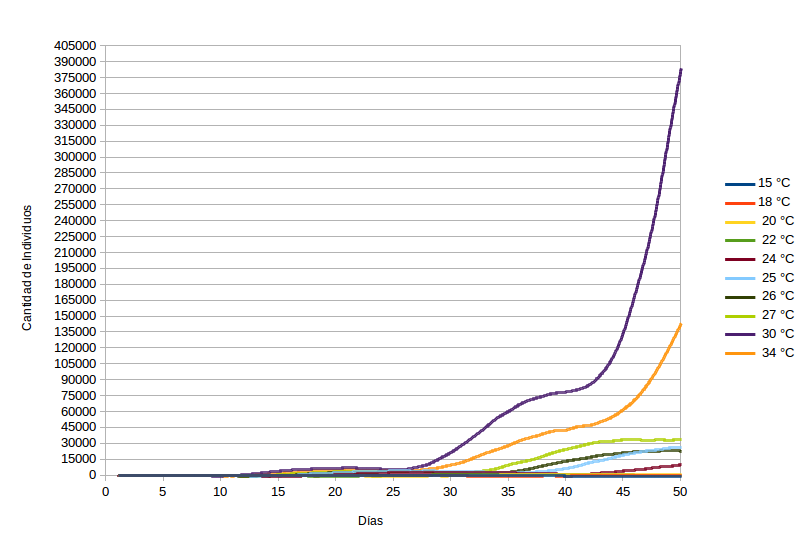
\includegraphics[width=\textwidth]{./graphics/evolucion-poblacion-all.png}
        \caption{ Población de mosquitos en etapas inmaduras.}
    \end{subfigure}
    ~~~~
    \begin{subfigure}[b]{0.45\textwidth}
        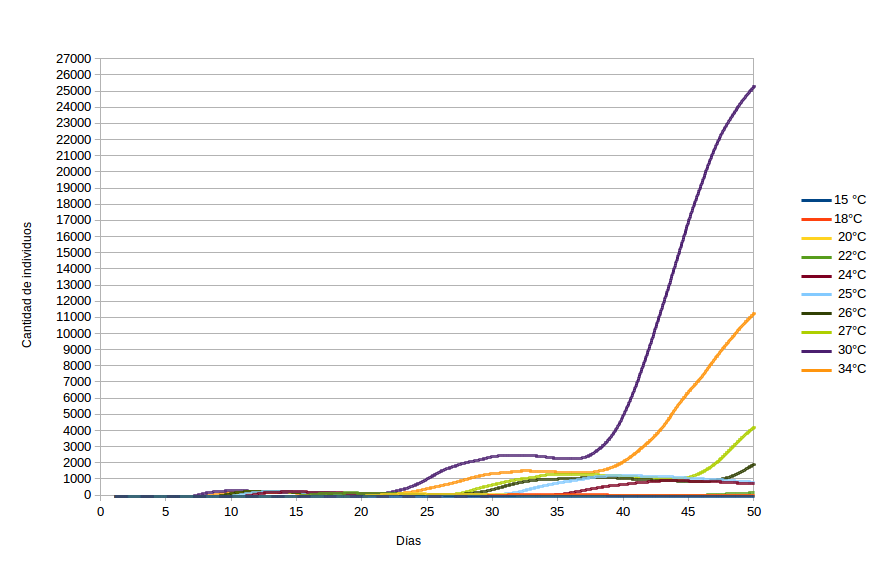
\includegraphics[width=\textwidth]{./graphics/evolucion-poblacion-adultos.png}
        \caption{ Población mosquitos adultos.}
    \end{subfigure}

\caption{\label{fig:poblacion-all}Análisis del comportamiento de la población de mosquitos en relación al tiempo a 10 temperaturas constantes (15-34 \textcelsius)}
\end{figure}

En la \figref{fig:poblacion-all} se puede apreciar el crecimiento y decrecimiento de la población
a diferentes temperaturas, en donde se pudo observar que a medida que la temperatura aumenta, las
tasas de desarrollo son menores, motivo por el cual las poblaciones de individuos en etapas
inmaduras, sometidos a temperaturas más elevadas, tienden a disminuir su tamaño rápidamente debido
a que se desarrollan con mayor rapidez, dando lugar a su etapa de adulto. Del mismo modo el ciclo
gonotrófico, para las hembras adultas tienden a disminuir su duración, causando que el intervalo
entre oviposturas disminuya, en consecuencia el tamaño de la población de individuos en etapas
inmaduras aumenta rápidamente.

\begin{figure}[!t]
    \centering
    \begin{subfigure}[b]{0.225\textwidth}
        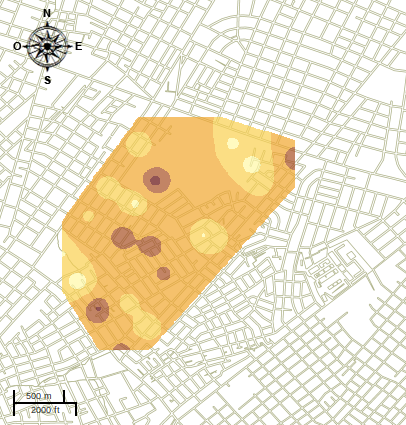
\includegraphics[width=\textwidth]{./graphics/inicial.png}
        \caption{ Población población inicial.}
    \end{subfigure}
    ~~~~
    \begin{subfigure}[b]{0.225\textwidth}
        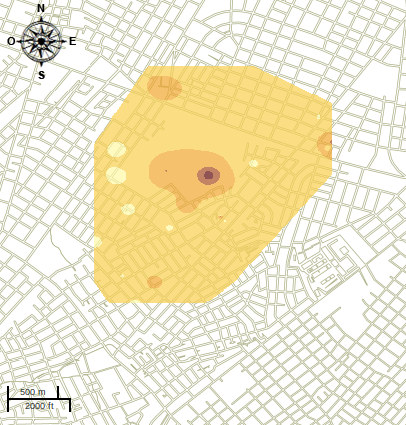
\includegraphics[width=\textwidth]{./graphics/temp-20-final.png}
        \caption{ Población final a 20 \textcelsius.}
    \end{subfigure}

    \begin{subfigure}[b]{0.225\textwidth}
        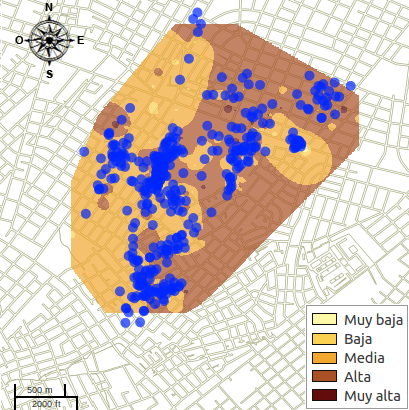
\includegraphics[width=\textwidth]{./graphics/temp-24-final.png}
        \caption{ Población final a 24 \textcelsius.}
    \end{subfigure}
    ~~~~
    \begin{subfigure}[b]{0.225\textwidth}
        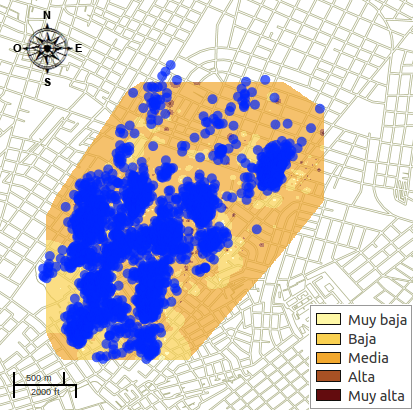
\includegraphics[width=\textwidth]{./graphics/temp-27-final.png}
        \caption{ Población final a 27 \textcelsius.}
    \end{subfigure}

    \begin{subfigure}[b]{0.225\textwidth}
        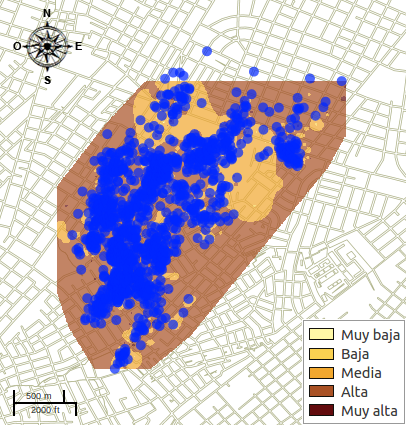
\includegraphics[width=\textwidth]{./graphics/temp-30-final.png}
        \caption{ Población final a 30 \textcelsius.}
    \end{subfigure}
    ~~~~
    \begin{subfigure}[b]{0.225\textwidth}
        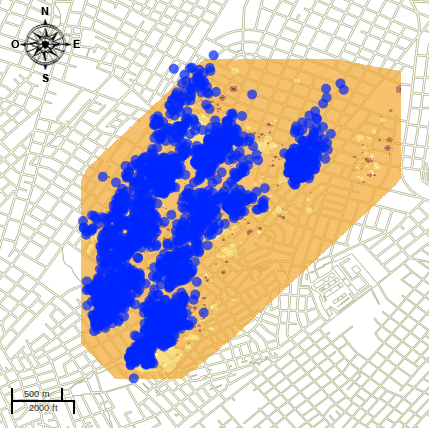
\includegraphics[width=\textwidth]{./graphics/temp-34-final.png}
        \caption{ Población final a 44 \textcelsius.}
    \end{subfigure}
\caption{\label{fig:poblacion-mapas-all} Mapas de interpolación de la población de mosquitos y la distribución de las hembras adultas (puntos en azul).}
\end{figure}

En la \figref{fig:poblacion-mapas-all} se puede apreciar los mapas de interpolación de las
poblaciones en un su estado inicial y final del periodo de simulación. El estado inicial es el
mismo para todas las temperaturas. Comparando el estado inicial y los estados finales se puede
observar que existe una dispersión de los focos en dirección al noreste debido a que la dirección
del viento utilizada era de sureste. Este patrón de dispersión se podrá observar en todas las
poblaciones que fueron sometidas a temperaturas que permitan la generación de hembras adultas. La
dispersión de los focos de infestación es consecuencia de la dispersión y ovipostura de las
hembras adultas emergentes de la población.


%conclusión final
\section{Conclusión}
%(1) Diseñar un modelo que permita analizar la extensión del vector del dengue y estudiar su posible relación con un potencial foco de riesgo, de forma a realizar una predicción de posibles focos de riesgo.
En este trabajo presentó el diseño e implementación de un modelo predictivo para identificar focos
de infestación del, Aedes aegypti principal vector del dengue, sustentado en métodos de muestreo
para la determinación de la abundancia poblacional, modelos matemáticos para simular el ciclo de
vida del vector en un sistema de información geográfica, con el fin de apoyar a la lucha
preventiva de esta enfermedad. Para el diseño y desarrollo del simulador del proceso evolutivo, se
realizaron ciertas consideraciones que requieren la validación y revisión por parte de expertos en
el área, de forma que se puedan realizar los ajustes correspondientes para su aplicabilidad.El diseño e implementación del modelo como un simulador del proceso evolutivo del vector en el contexto de un sistema de información geográfica, permite realizaranálisis complejos de la realidad espacial rápidamente, generando información regionalizada para determinar los niveles de infestación correspondientes al área de estudio. Se considera al modelo resultante como genérico, debido a que sus parámetros pueden ser ajustados para aplicarlos en cualquier región o área de estudio, y extensible, teniendo en cuenta que puede ser modificado para incluir nuevas variables y procesos.

%(3)Diseñar el modelo de forma paramétrica y escalable, para que sea aplicable y extensible a cualquier región o área de estudio.
El simulador de proceso evolutivo se encuentra compuesto por modelos, ampliamente respaldados por
el material bibliográfico, en \cite{sharpe1977reaction, focks1993dynamic, schoolfield1981non, otero2006stochastic, rueda1990temperature}, que son utilizados para el cálculo de las tasas de
desarrollo y mortalidad de las distintas etapas de desarrollo del ciclo de vida del vector. La
configuración del simulador del proceso evolutivo requiere de parámetros asociados con las
características biológicas y datos ecológicos correspondientes al área de estudio, por lo que para
su aplicación, estos parámetros de configuración deben ser validados por expertos en el área
mediante trabajos de campo. No obstante, utilizando valores tomados del material bibliográfico de
apoyo, se pudo observar un buen comportamiento de los resultados obtenidos mediante el simulador
del proceso evolutivo. Solo presentan pequeñas variaciones en comparación con los valores
observados por expertos en laboratorio en condiciones controladas. Las variaciones observadas
pueden ser causadas por los distintos rasgos característicos de las cepas de mosquitos, utilizadas
en los estudios de referencia, que permiten una mayor o menor tolerancia a ciertas condiciones.

%(4)Generar información relevante que pueda ayudar a las autoridades pertinentes para toma de decisiones en la lucha contra el dengue.
En un futuro, con los ajustes y validaciones correspondientes a ser realizadas por expertos en el
área, la información generada por el simulador del proceso evolutivo del Aedes aegypti, asociada
con niveles de infestación y los mapas de interpolación podrían, permitir a las autoridades
sanitarias, del Paraguay, definir y planificar, de forma más efectiva, las medidas de control,
prevención y logística a realizar con con el fin de disminuir los niveles de infestación en una
región.


% no \IEEEPARstart

% An example of a floating figure using the graphicx package.
% Note that \label must occur AFTER (or within) \caption.
% For figures, \caption should occur after the \includegraphics.
% Note that IEEEtran v1.7 and later has special internal code that
% is designed to preserve the operation of \label within \caption
% even when the captionsoff option is in effect. However, because
% of issues like this, it may be the safest practice to put all your
% \label just after \caption rather than within \caption{}.
%
% Reminder: the "draftcls" or "draftclsnofoot", not "draft", class
% option should be used if it is desired that the figures are to be
% displayed while in draft mode.
%
%\begin{figure}[!t]
%\centering
%\includegraphics[width=2.5in]{myfigure}
% where an .eps filename suffix will be assumed under latex,
% and a .pdf suffix will be assumed for pdflatex; or what has been declared
% via \DeclareGraphicsExtensions.
%\caption{Simulation Results}
%\label{fig_sim}
%\end{figure}

% Note that IEEE typically puts floats only at the top, even when this
% results in a large percentage of a column being occupied by floats.


% An example of a double column floating figure using two subfigures.
% (The subfig.sty package must be loaded for this to work.)
% The subfigure \label commands are set within each subfloat command, the
% \label for the overall figure must come after \caption.
% \hfil must be used as a separator to get equal spacing.
% The subfigure.sty package works much the same way, except \subfigure is
% used instead of \subfloat.
%
%\begin{figure*}[!t]
%\centerline{\subfloat[Case I]\includegraphics[width=2.5in]{subfigcase1}%
%\label{fig_first_case}}
%\hfil
%\subfloat[Case II]{\includegraphics[width=2.5in]{subfigcase2}%
%\label{fig_second_case}}}
%\caption{Simulation results}
%\label{fig_sim}
%\end{figure*}
%
% Note that often IEEE papers with subfigures do not employ subfigure
% captions (using the optional argument to \subfloat), but instead will
% reference/describe all of them (a), (b), etc., within the main caption.


% An example of a floating table. Note that, for IEEE style tables, the
% \caption command should come BEFORE the table. Table text will default to
% \footnotesize as IEEE normally uses this smaller font for tables.
% The \label must come after \caption as always.
%
%\begin{table}[!t]
%% increase table row spacing, adjust to taste
%\renewcommand{\arraystretch}{1.3}
% if using array.sty, it might be a good idea to tweak the value of
% \extrarowheight as needed to properly center the text within the cells
%\caption{An Example of a Table}
%\label{table_example}
%\centering
%% Some packages, such as MDW tools, offer better commands for making tables
%% than the plain LaTeX2e tabular which is used here.
%\begin{tabular}{|c||c|}
%\hline
%One & Two\\
%\hline
%Three & Four\\
%\hline
%\end{tabular}
%\end{table}


\printbibliography

% that's all folks
\end{document}


